% $Id%

\pagebreak
\enlargethispage{1cm}
\section{CrypTool Menus}
\hypertarget{appendix-menutree}{}\label{s:appendix-menutree}
This appendix contains the complete menu tree of CrypTool. 
Please notice that not all menu items are always available, because the
menu tree is built up dynamically: which menu items are available depends
on the type of the currently active document window.
The brute-force analysis for DES e.~g. is only available, if the active
window is opened in the hexadecimal view. On the other hand the menu item
"`Generate Random Numbers\dots"' is always available. 
Within the figures \ref{menu-detail-1} and \ref{menu-detail-2} 
this relation is shown in the brackets after the menu items,
e.~g. "`Find\dots[ATH]"' means, that the function "`Find\dots"' is only
available for ASC-, text- and hexadecimal windows.
\begin{center}
\begin{tabular}{rl}
\bf Code letter & \bf Type of document \\
M & (no document opened)\\
A & ASC\\
T & Text\\
H & Hexadecimal\\
P & Plot\\
\end{tabular}
\end{center}

\nobreak

\begin{figure}[!hb]
\begin{center}
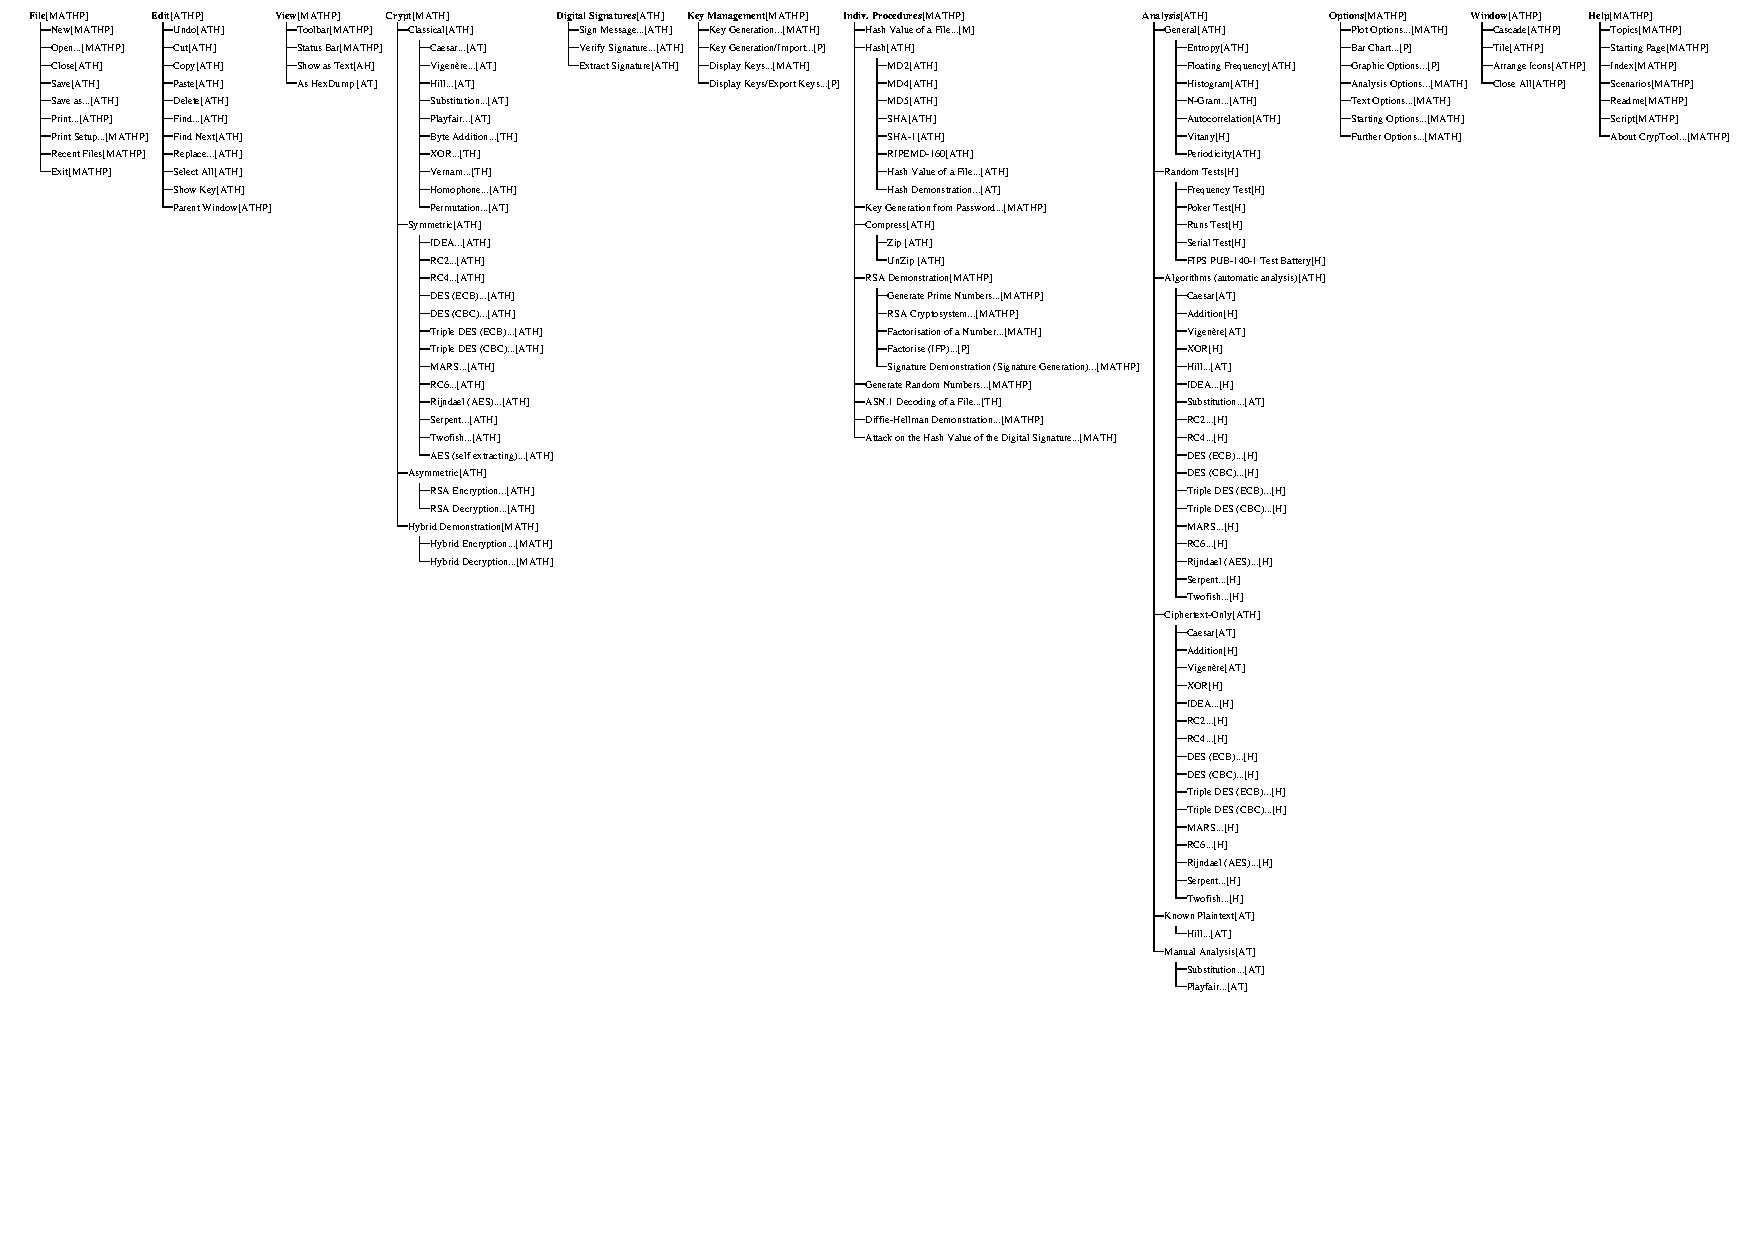
\includegraphics[scale=1.1, clip, viewport=10 360 400 600]{figures/cryptool-menu-detail-en}
\caption{Detailled view of the CrypTool menu tree -- part 1}
\label{menu-detail-1}
\end{center}
\end{figure}

\begin{figure}[b]
\begin{center}
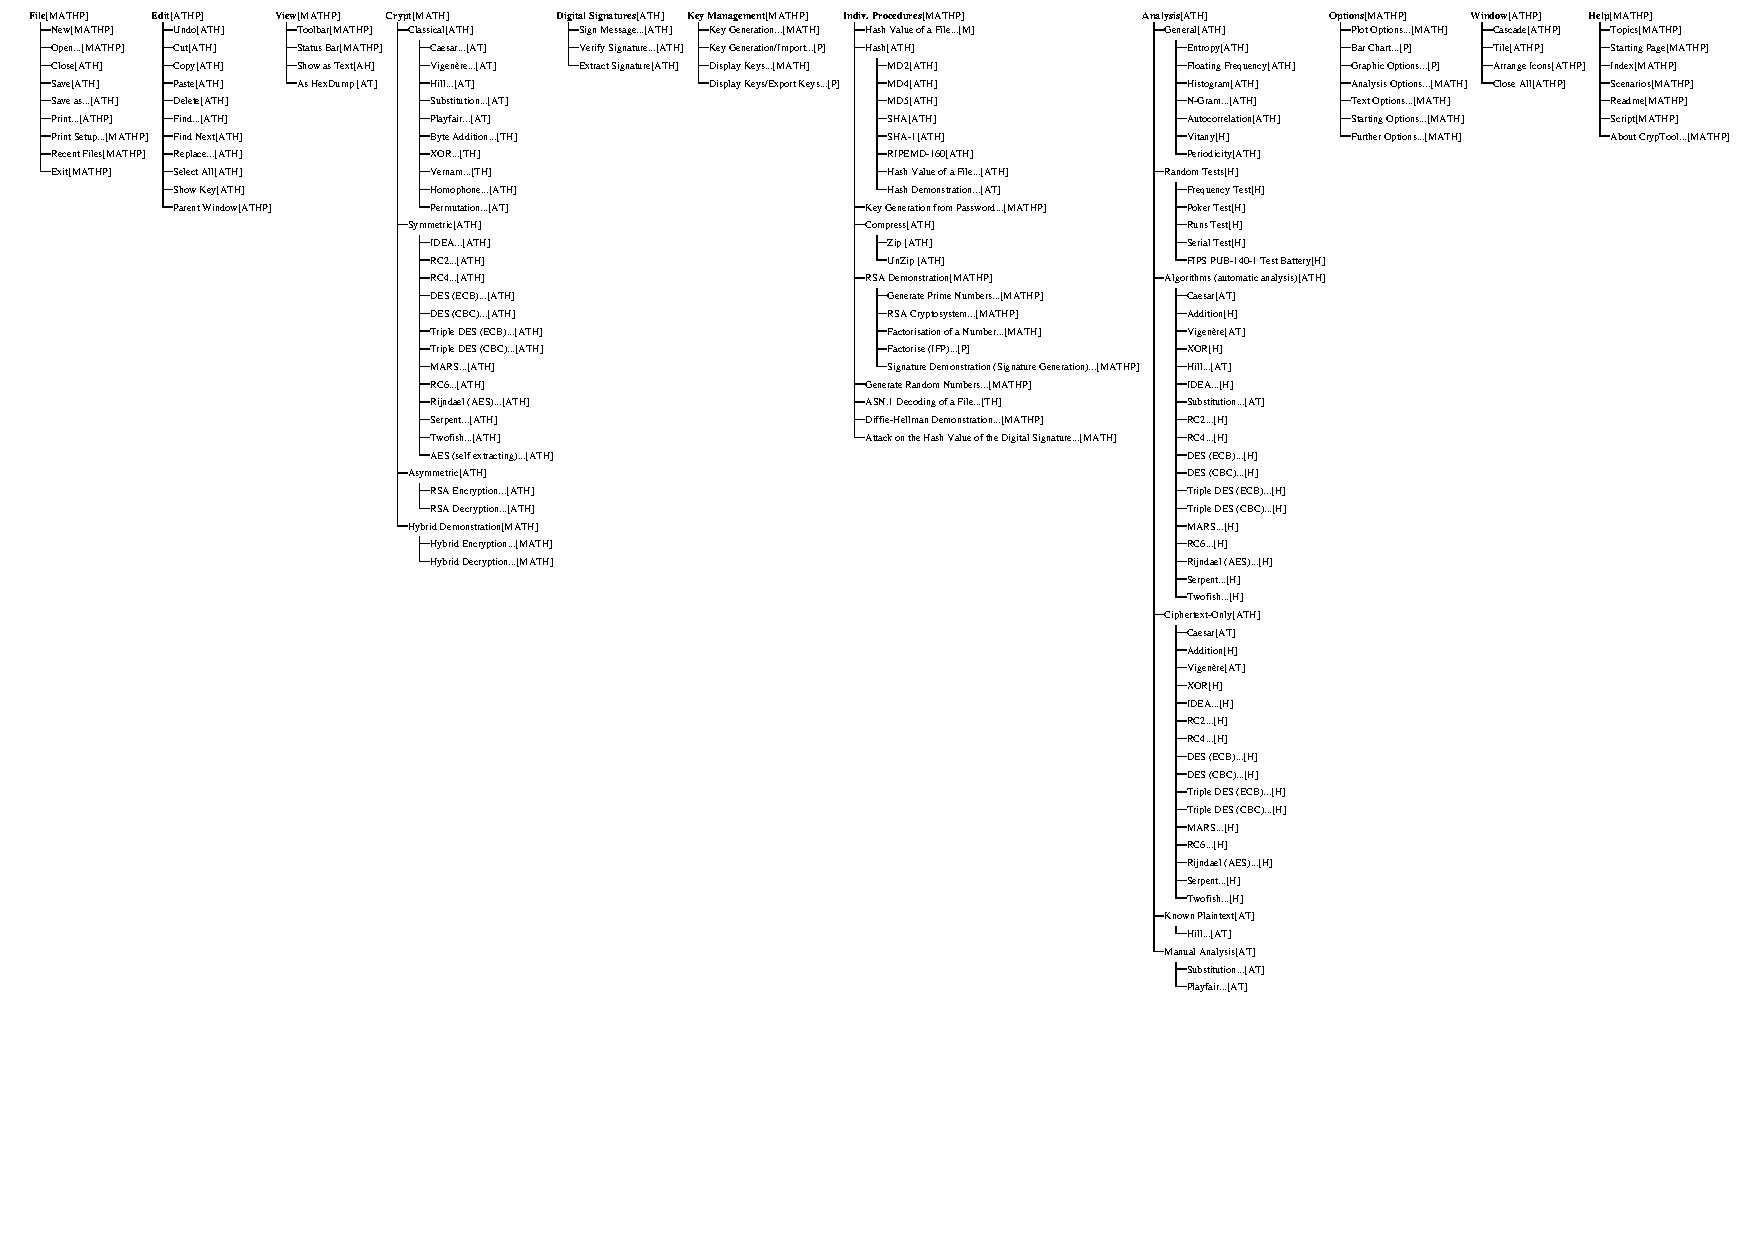
\includegraphics[scale=1.1, clip, viewport=400 190 784 598]{figures/cryptool-menu-detail-en}
\caption{Detailled view of the CrypTool menu tree -- part 2}
\label{menu-detail-2}
\end{center}
\end{figure}

\begin{figure}[hb]
\begin{center}
\includegraphics[scale=0.75, angle=270, viewport=14 107 779 590]{figures/cryptool-menu-en}
\vspace{-18pt}
\caption{Complete Overview of the CrypTool menu tree} 
\label{menuoverview}
\end{center}
\end{figure}
